\documentclass[a4,12pt]{article}
\setlength{\headsep}{-1.cm}
\setlength{\textheight}{24cm}
\setlength{\oddsidemargin}{-.5cm}
\setlength{\evensidemargin}{-.5cm}
\setlength{\textwidth}{17.cm}
\setlength{\footskip}{1.cm}
\usepackage[T1]{fontenc}
\usepackage{color}


\usepackage[utf8]{inputenc}

%\pagestyle{empty}

\usepackage{graphicx}

\begin{document}
  
\noindent
\begin{center}
\textbf{\large TP num\'erique: Dynamique des Fluides}\\
\textbf{ Inspir\'e du TD: "Rythmes cardiaques"}
\end{center}

\bigskip

L'objectif de ce TP est d'approximer num\'eriquement un \'ecoulement induit entre deux plans par un gradient 
de pression oscillant.
Ce type de probl\`eme peut mod\'eliser la mani\`ere dont les battements du c{\oe}ur induisent un 
\'ecoulement puls\'e dans les vaisseaux sanguins.
En effet ces battements imposent une variation p\'eriodique du gradient de pression impos\'e 
entre deux sections transverses des vaisseaux.
L'objectif de cet exercice est de caract\'eriser ce type d'\'ecoulement
en particulier dans les limites des basses fr\'equences (organisme au repos) 
et hautes fr\'equences (activit\'e cardiaque intense).

Consid\'erons un mod\`ele d'\'ecoulement plan entre deux plaques
planes distantes de $2h$, g\'en\'er\'e par un gradient de pression
sinuso\"{\i}dal \`a pulsation $\omega$ fix\'ee~:
\[
\frac{dp}{dx} = K \cos\omega t.
\]
\noindent
Ici $K$ correspond à l'amplitude du gradient de pression impos\'e.
\begin{figure}[htb]
  \begin{center}
    \setlength{\unitlength}{1mm}
    \begin{picture}(60, 40)(0, 0)
      \put(0, 0){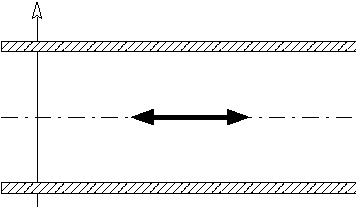
\includegraphics[width=6cm]{ecoulement_pulse}}
      \put(0, 6){$-h$}
      \put(0, 22){$+h$}
      \put(20, 20){$\partial p/\partial x = K \cos \omega t$}
    \end{picture}
  \end{center}
  \caption{\'Ecoulement puls\'e en conduite.}
  \label{fig:ecoulement_pulse}
\end{figure}
\section{Visulation de la solution analytique (en régime établi)}
\begin{enumerate}
\item Dans l'hypoth\`ese d'un \'ecoulement plan parall\`ele, et d'une vitesse $u$ nulle sur les 
parois inf\'erieure et sup\'erieure,
 montrer que
la vitesse horizontale $u(y, t)$ v\'erifie l'\'equation:
\begin{equation}
\label{par}
  \frac{\partial u}{\partial t} 
  = 
  - \frac{K}{\rho} \cos \omega t + \nu \frac{\partial^2 u}{\partial y^2}
  \label{eq:ns}
\end{equation}

\noindent
Sous l'hypothèse d'un {\em régime établi}, le problème admet une solution analytique. Le forçage étant de la forme $\cos \omega t $ on peut rechercher la solution sous la forme $u(y,t) = u_c(y) \cos \omega t + u_s(y) \sin(\omega t)$. Il est cependant plus efficace d'utiliser la méthode de la variable complexe en posant $u_{th}(y, t) = Re \left \{ \underline{U}(y) e^{i \omega t} \right \}$ où $\underline{U}(y) = u_c(y) - i u_s(y)$ est une fonction à valeur complexe. En remplaçant $\cos \omega t$ par $e^{i\omega t}$  dans l'\'equation~(\ref{eq:ns}), et en cherchant la solution vérifiant les conditions limites $u(\pm h,t) = 0$, on obtient finalement l'expression du profil de vitesse instationnaire suivant~:
\begin{equation}
\label{sol}
 \underline{U}(y) = \frac{iK}{\rho \omega} \left \{ 
1 - \frac{\cosh [ y ( 1+i) \sqrt{\omega / 2\nu} ]}{\cosh [ 
h ( 1+i) \sqrt{\omega / 2\nu} ]}
\right \}
\end{equation}
\item Retrouver les solutions (\ref{sol}) \`a partir de l'\'equation (\ref{par}).

\item La solution complète du problème est la solution établie précédente,
plus une solution particulière sans second membre, qui correspond à un
régime transitoire amorti et qui dépend des conditions
initiales. 

Estimez le temps caractéristique $\tau$ d'amortissement de ce transitoire.
 
%%% Pauline : tau = h^2/nu par analyse dimensionnelle de l'équation sans second membre

\item En adimensionnant $t$ et $y$ respectivement par $1/\omega$
et $h$ la solution se met sous la forme :
\begin{equation}
\label{soladim}
 \underline{U}^\star(y^\star) = \frac{i\gamma}{\Omega^2} \left \{
1 - \frac{\cosh [ y^\star ( 1+i) \sqrt{\Omega} ]}{\cosh [ 
( 1+i) \sqrt{\Omega} ]} \right \}
\quad
\mbox{avec} \quad
\Omega = \frac{\omega h^2}{2\nu}, \; \gamma = \frac{Kh^3}{4\rho \nu^2}
\end{equation}
\noindent 
avec $^\star$ exprimant le fait que ces variables sont adimensionn\'ees. 

On fournit un programme \textsc{Matlab} \texttt{pulse.m} qui permet de visualiser
cette solution théorique. A l'aide de ce programme visualiser les profils de vitesse pour différentes valeurs de $\Omega$ prises dans l'intervalle $10^{-3} \leq \Omega <10^3$.

Repr\'esenter sch\'ematiquement sur votre compte-rendu la forme du profil de vitesse
à différents instants du cycle, dans les deux r\'egimes asymptotiques des grands et petits $\Omega$.
Commentez physiquement les résultats.

\item  D'apr\`es vous que repr\'esente physiquement le param\`etre $\Omega$ ? 


\end{enumerate}

\section{Calcul num\'erique}
On propose de r\'esoudre num\'eriquement cette \'equation de diffusion 
1D instationnaire forc\'ee.
Ceci permettra d'une part de comparer l'approximation numérique avec
la solution théorique en régime établi, et d'autre part d'observer
le régime transitoire précédent la convergence vers ce régime établi.

 La solution num\'erique est calcul\'ee en utilisant des m\'ethodes aux diff\'erences finies.


La discrétisation spatiale est effectuée en introduisant $N_y$ points intérieurs au domaine et définis
par $y_i = (i \Delta y -h)$ avec $i=1..N_y$ et $\Delta y = 2 h /(N_y+1)$.

La discrétisation temporelle est effectuée en posant  $t^{(n)}=n\Delta t$ avec $n=0,..,N_t$.

Enfin, on pose $u_i^{(n)} = u(y_i,t^{(n)})$.

Le sch\'ema utilis\'e sera un Euler explicite d'ordre 1 en temps, et des diff\'erences finies centr\'ees d'ordre 2 en espace.
En utilisant ce schéma l'\'equation (\ref{par}) prend la forme:
\begin{equation}
\label{disc}
\frac{u_i^{(n+1)}-u_i^{(n)}}{\Delta t}=-\frac{K}{\rho} \cos( \omega t^{(n)} ) + \frac{\nu}{\Delta y^2} 
\left[ u_{i+1}^{(n)}-2u_i^{(n)}+u_{i-1}^{(n)} \right] 
\end{equation}
\noindent


Remarquons que les $y_i$ d\'ecrivent les points \`a l'int\'erieur du domaine, et du fait des conditions aux limites 
de non-glissement impos\'ees sur les parois on a $u(y_0,t^{(n)})=u(y_{N_y+1},t^{(n)})=0, \ \forall n$.

Pour la résolution numérique deux stratégies sont possibles :
\begin{itemize}
\item 
On peut construire un tableau à deux dimensions \verb| U(i,n)| contenant toutes les valeurs $u_{i}^{(n)}$, et remplir les unes après les autres les colonnes du tableau correspondant aux valeurs de $u$ aux instants successifs. L'inconvénient est de nécessiter un important stockage de mémoire, inutile si l'on ne s'intéresse qu'à l'état final.
\item 
En notant que le schéma ne fait intervenir que la solution à deux pas de temps successifs, on peut se contenter d'utiliser seulement deux vecteurs colonnes 
\verb| Ufutur | et \verb| Upresent |  contenant à chaque pas de temps les valeurs à l'instant 
"présent" $t^{(n)}$ et "futur"  $t^{(n+1)}$ (c.a.d. $ U^{present} = [u_1^{(n)}; u_2^{(n)}; ... u_{N_y}^{(n)} ] $ et   $U^{futur} = [u_1^{(n)}; u_2^{(n)}; ... u_{N_y}^{(n)}$).
\end{itemize}


\begin{enumerate}
\item Montrez qu'avec cette seconde idée le calcul de la solution à chaque itération temporelle se met sous la forme :
\begin{equation}
\label{mat}
U^{futur} =A\, U^{present} +F cos(\omega t^{n}).
\end{equation}
\noindent
Où $A$ est une matrice carrée correspondant 
\`a la discr\'etisation de l'op\'erateur Laplacien et $F$ est un vecteur colonne 
repr\'esentant le terme de for\c{c}age. Pr\'eciser les dimensions des
matrices et vecteurs mis en jeu dans (\ref{mat}). 

\item Ecrire un programme effectuant l'intégration temporelle du problème,
en fonction des différents paramètres physiques et numériques,
en partant de la condition initiale $u(x,t=0) = 0$, et jusqu'à un instant final $t_f$.


Dans votre comte-rendu, vous détaillerez la stratégie de programmation utilisée.

\item A l'aide de votre programme, calculez et tracez la solution numérique obtenue 
à un instant correspondant à {\color{red} une période du forçage (c.a.d. $t_f = 2\pi / \omega$)}
%où $\tau$ est le temps caractéristique
%déterminé précédemment, 
avec les paramètres donnés dans le tableau:
$$
\begin{array}{|c|c|c|c|c|}
\hline
h & K/\rho & \nu & \omega & N_y \\
\hline
\hspace{2cm} & \hspace{2cm} & \hspace{2cm} & \hspace{2cm} & 100 \\
\hline
\end{array}
$$
Vous déterminerez vous-même une valeur de $\Delta t$ à utiliser pour aboutir
à un bon compromis entre précision et temps de calcul.

%%% PAULINE : la condition de stabilité théorique est delta t / (delta y)^2 < 1/2

\item Qu'observe-t-on avec des valeurs de $\Delta t$ trop grandes ? Expliquez.

\item Tracez sur le même graphique la solution théorique $u_{th}(y,t_f)$.
Commentez les différences.

\item Calculez maintenant à l'aide de votre programme la solution 
correspondant à l'instant {\color{red} $t_f = 10 (2\pi /\omega)$} et comparez avec la solution théorique. Commentez.


\item R\'e\'ecrire le sch\'ema (\ref{disc}) de mani\`ere implicite avec un schéma de Cranck-Nicholson.
(c'est-\`a-dire que la discr\'etisation du laplacien est exprim\'ee au temps $n+1/2$, défini comme 
moyenne des valeurs aux instants $n$ et $n+1$). Précisez l'ordre de ce schéma, et le traitement 
choisi pour le second membre de l'équation différentielle.

%%% PAULINE : prendre $cos ( \omega t^{n+1/2} ) $ pour être cohérent 

Ecrire ce nouveau schéma sous forme matricielle. 

\item Ecrire un nouveau programme effectuant l'intégration numérique de ce nouveau schéma.

\item Toujours pour les paramètres donnés dans le tableau et pour $t_f = 10 (2\pi/\omega)$, tracez et imprimer la solution numérique obtenue pour plusieurs valeurs de $\Delta t$. Comparez ces résultats à ceux obtenus avec le schéma explicite, et discutez en terme de précision, de stabilité, 
et de temps de calcul.


\clearpage





\fontfamily{cmss}\fontshape{n}\selectfont
\fontfamily{cmss}\fontshape{n}\selectfont



%~\\

\noindent 

\begin{center}
{\Large PLANNING DES SEANCES (2018)}
\end{center}
\noindent


{\bf Groupe 1 :} vendredi 2 février, 13h30-16h30

{\bf Groupe 2 :} vendredi 9 février, 13h30-16h30

{\bf Groupe 3 :} vendredi 9 février, 16h30-19h30 

\noindent
Les étudiants ayant déjà validé des TPs l'année dernière devront se présenter lors de la première séance pour faire connaitre leurs intentions à l'enseignant.

~\\
%\clearpage
\begin{center}
{\Large CONSIGNES POUR LA REDACTION DES COMPTES-RENDUS}
\end{center}
\noindent
Le compte-rendu sera réalisé par groupes de deux personnes.

\noindent
Le rapport ne doit pas excéder 4 feuilles recto-verso hors courbes. 
Il devra présenter le problème physique concerné, la modélisation numérique utilisée, 
la stratégie de programmation utilisée et les résultats obtenus. Dans la présentation on  veillera a distinguer les aspects de validation numérique (précision, convergence, etc...) des résultats physiques. 
Le rapport devra également indiquer les éventuelles difficultés rencontrées dans la mise en place ainsi que l'état d'avancement par rapport aux objectifs du TP. 
 
\noindent
 Les figures devront \^etre numérotées, citées et commentées dans le texte. Chaque figure doit obligatoirement comporter un titre clair (ou une légende située sous la figure), et les axes doivent être gradués et identifiés. (vous pouvez utiliser les commandes matlab \verb| title, xlabel|,
 \verb| ylabel | ).

Toute figure incomplète ne sera pas considérée dans la note.

{\color{red} Le programme écrit devra être fourni en annexe du rapport, ou déposé sur MOODLE comme un document séparé. 
}


\noindent
Le rapport débutera par une introduction fixant les objectifs. 
Vous pouvez terminer votre rapport par des remarques de synthèse. 

~\\

\begin{center}
{\Large PROCEDURE DE DEPOT DES COMPTES-RENDUS}\\
~\\

Les comptes-rendus seront à rendre SUR MOODLE, au plus tard 2 semaines après 
la séance de TP (vendredi 16 février pour le groupe 3, vendredi 23 février pour les groupes 1-2).

Si le rapport a été rédigé par ordinateur, inutile de rendre une version papier.

Si le rapport a été rédigé à la main, vous devrez scanner (ou prendre en photo) le rapport pour le déposer sur moodle, et rendre également une version papier au cours suivant.







~
~\\


\begin{center}
{\large IL EST RAPPELE QUE LES TPS SONT OBLIGATOIRES.}
\end{center}

\end{center}






\end{enumerate}


\end{document}
